\documentclass{article}
\usepackage[margin=1in]{geometry}
\usepackage{amsmath,amsthm,amssymb}
\usepackage{bbm,enumerate,mathtools}
\usepackage{tikz,pgfplots}
\usepackage{chessboard}
\usepackage[hidelinks]{hyperref}
\usepackage{multicol} % Problem 35

\newenvironment{question}{\begin{trivlist}\item[\textbf{Question.}]}{\end{trivlist}}
\newenvironment{note}{\begin{trivlist}\item[\textbf{Note.}]}{\end{trivlist}}
\newenvironment{references}{\begin{trivlist}\item[\textbf{References.}]}{\end{trivlist}}
\newenvironment{related}{\begin{trivlist}\item[\textbf{Related.}]\end{trivlist}\begin{enumerate}}{\end{enumerate}}


\begin{document}

\rating{3}{3}
According to F\'ary's theorem, any planar graph can be drawn as a planar
straight-line graph. This problem studies which of these straight-line graphs are the smallest.

Given a planar graph $G$ let $S_G$ be the set of all
straight-line embeddings of $G$ where the shortest edge has length $1$.
Given an embedding $E$, let $\ell(E)$ be the average edge length, and let $f(G) = \inf\{\ell(E) : E \in S_G\}$.

\begin{figure}[ht!]
  \centering
  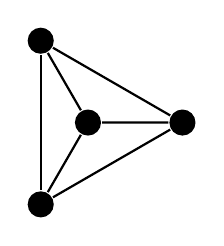
\begin{tikzpicture}[scale=1.2]
    \node[shape=circle, fill, thick] (v1) at (0,0) {};
    \node[shape=circle, fill, thick] (v2) at (0,{sqrt(3)}) {};
    \node[shape=circle, fill, thick] (v3) at (1/2,{sqrt(3)/2}) {};
    \node[shape=circle, fill, thick] (v4) at (3/2,{sqrt(3)/2}) {};
    \draw[thick]
      (v1) edge (v2)
      (v1) edge (v3)
      (v1) edge (v4)
      (v2) edge (v3)
      (v2) edge (v4)
      (v3) edge (v4)
    ;
  \end{tikzpicture}
  ~~~
  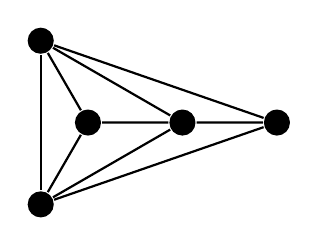
\begin{tikzpicture}[scale=1.2]
    \node[shape=circle, fill, thick] (v1) at (0,0) {};
    \node[shape=circle, fill, thick] (v2) at (0,{sqrt(3)}) {};
    \node[shape=circle, fill, thick] (v3) at (1/2,{sqrt(3)/2}) {};
    \node[shape=circle, fill, thick] (v4) at (3/2,{sqrt(3)/2}) {};
    \node[shape=circle, fill, thick] (v5) at (5/2,{sqrt(3)/2}) {};
    \draw[thick]
      (v1) edge (v2)
      (v1) edge (v3)
      (v1) edge (v4)
      (v1) edge (v5)
      (v2) edge (v3)
      (v2) edge (v4)
      (v2) edge (v5)
      (v3) edge (v4)
      (v4) edge (v5)
    ;
  \end{tikzpicture}
  \caption{Conjectured minimal embeddings showing $\displaystyle f(K_4) \leq \frac{3\sqrt{3} + 3}6$ and
  $\displaystyle f(K_5 \setminus \{e\}) \leq \frac{3\sqrt{3} + 4 + \sqrt{28}}9$.}
\end{figure}

\begin{figure}[ht!]
  \centering
  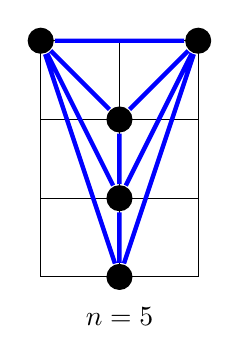
\begin{tikzpicture}
    \draw (0,0) grid (2,3);
    \node[shape=circle, fill, thick] (v1) at (0,3) {};
    \node[shape=circle, fill, thick] (v4) at (2,3) {};
    \node[shape=circle, fill, thick] (v2) at (1,1) {};
    \node[shape=circle, fill, thick] (v3) at (1,2) {};
    \node[shape=circle, fill, thick] (v5) at (1,0) {};
    \draw[ultra thick, blue]
      (v1)--(v2)--(v3)--(v1)--(v4)--(v2)
      (v3)--(v4)--(v5)
      (v1)--(v5)--(v2)
    ;
    \node at (1, -1/2) {$n = 5$};
  \end{tikzpicture}
  ~~~
  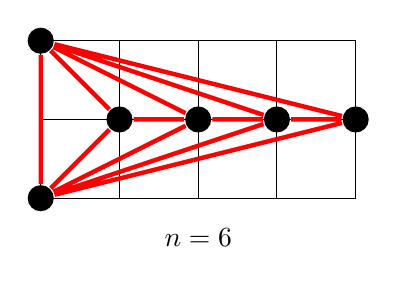
\begin{tikzpicture}
    \draw (0,0) grid (4,2);
    \node[shape=circle, fill, thick] (v1) at (0,0) {};
    \node[shape=circle, fill, thick] (v2) at (0,2) {};
    \node[shape=circle, fill, thick] (v3) at (1,1) {};
    \node[shape=circle, fill, thick] (v4) at (2,1) {};
    \node[shape=circle, fill, thick] (v5) at (3,1) {};
    \node[shape=circle, fill, thick] (v6) at (4,1) {};
    \draw[ultra thick, red]
      (v1)--(v2)--(v3)--(v1)--(v4)--(v2)--(v5)--(v1)--(v6)--(v2)
      (v3)--(v4)--(v5)--(v6)
    ;
    \node at (2, -1/2) {$n = 6$};
  \end{tikzpicture}
  ~~~
  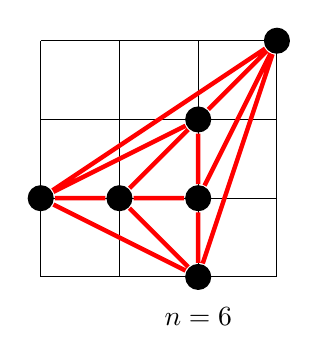
\begin{tikzpicture}
    \draw (0,0) grid (3,3);
    \node[shape=circle, fill, thick] (v1) at (0,1) {};
    \node[shape=circle, fill, thick] (v2) at (1,1) {};
    \node[shape=circle, fill, thick] (v3) at (2,2) {};
    \node[shape=circle, fill, thick] (v4) at (2,0) {};
    \node[shape=circle, fill, thick] (v5) at (2,1) {};
    \node[shape=circle, fill, thick] (v6) at (3,3) {};
    \draw[ultra thick, red]
      (v2)--(v3)--(v5)--(v2)
      (v1)--(v3)--(v6)--(v1)
      (v1)--(v4)--(v2)--(v1)
      (v4)--(v5)--(v6)--(v4)
    ;
    \node at (2, -1/2) {$n = 6$};
  \end{tikzpicture}
  \caption{Smallest (?) grids that contain all planar simple graphs on $n$ vertices are $[3] \times [4]$ for $n=5$ and $[5] \times [4]$ for $n=6$.}
\end{figure}

\begin{question}
  Given some graph $G$, what is $f(G)$?
\end{question}

\begin{related}
  \item How does $\max\{f(G) : G \text{ is planar with } n \text{ vertices}\}$ grow with respect to $n$?
  \item What if the vertices must be on $\mathbb Z^2$? What is the smallest
    square that can contain all planar graphs with $n$ vertices?
  \item What is the smallest $nmk$ such that $K_n$ can be drawn in
    $[n] \times [m] \times k$ with straight-line edges and no edges intersecting?
  \item Is it always possible to write a planar graph as a straight-line graph
    with integer edge lengths? If not, when is this possible? If so, what's the
    minimal edge sum?
  \item What is the longest non-self-intersecting polygonal chain that can fit
    in an $n \times m$ grid?
  \item What is the supremum of $\ell(E)$ over all  straight-line embeddings with longest edge \textit{at most} $1$? Are these just rescalings of the original case?
\end{related}

\begin{references}
  \item Problem 74.
  \item Problem 85.
  \item \url{https://oeis.org/A000109}
\end{references}
\end{document}
